\documentclass[tikz,border=5pt]{standalone}
\usepackage{amsmath}
\usetikzlibrary{arrows.meta,calc}
\tikzset{axis/.style={-{Stealth[length=2mm]},thin},force/.style={-{Stealth[length=2.4mm]},very thick},
track/.style={blue!65!black,line width=1.2pt},point/.style={circle,fill=black,inner sep=1.6pt}}
\begin{document}
% statement-03: illustration l=3, theta0=55 deg; no answer curve in the statement.
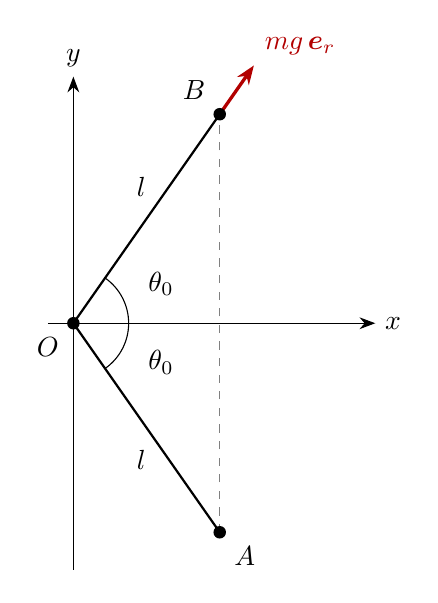
\begin{tikzpicture}[scale=1.08]
\def\ll{3}\def\ang{55}
\coordinate (O) at (0,0);
\coordinate (A) at ({\ll*cos(\ang)},{-\ll*sin(\ang)});
\coordinate (B) at ({\ll*cos(\ang)},{\ll*sin(\ang)});
\draw[axis] (-.3,0)--(3.55,0) node[right] {$x$};
\draw[axis] (0,-2.9)--(0,2.9) node[above] {$y$};
\draw[thick] (A)--(O)--(B);
\draw[gray,dashed] (A)--(B);
\draw (0.65,0) arc[start angle=0,end angle=\ang,radius=.65];
\draw (0.65,0) arc[start angle=0,end angle=-\ang,radius=.65];
\node at (1.03,.46) {$\theta_0$};\node at (1.03,-.46) {$\theta_0$};
\node[above left] at ($(O)!.56!(B)$) {$l$};
\node[below left] at ($(O)!.56!(A)$) {$l$};
\draw[force,red!70!black] (B)--++({.7*cos(\ang)},{.7*sin(\ang)}) node[above right] {$mg\,\boldsymbol e_r$};
\node[point,label=below left:$O$] at (O) {};
\node[point,label=below right:$A$] at (A) {};
\node[point,label=above left:$B$] at (B) {};
\end{tikzpicture}

% element-03: enlarged differential triangle in the local outward radial/tangential frame.
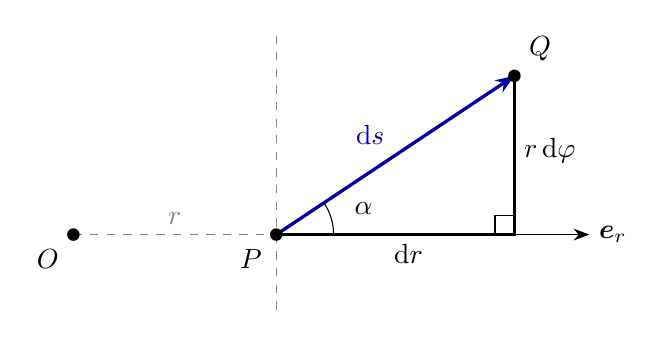
\begin{tikzpicture}[scale=1.12]
\coordinate (O) at (-2.3,0);\coordinate (P) at (0,0);
\coordinate (H) at (2.7,0);\coordinate (Q) at (2.7,1.8);
\draw[gray,dashed] (O)--(P) node[midway,above] {$r$};
\draw[axis] (P)--(3.55,0) node[right] {$\boldsymbol e_r$};
\draw[gray,dashed] (0,-.85)--(0,2.3);
\draw[thick] (P)--(H)--(Q);
\draw[force,blue!65!black] (P)--(Q) node[midway,above left] {$\mathrm ds$};
\draw (.65,0) arc[start angle=0,end angle=33.6901,radius=.65];
\node at (.99,.29) {$\alpha$};
\draw (2.48,0)--(2.48,.22)--(2.7,.22);
\node[below] at (1.5,0) {$\mathrm dr$};
\node[right] at (2.7,.95) {$r\,\mathrm d\varphi$};
\node[point,label=below left:$O$] at (O) {};
\node[point,label=below left:$P$] at (P) {};
\node[point,label=above right:$Q$] at (Q) {};
\end{tikzpicture}

% parabola-03: l=3.6, theta0=60 deg, c=2.7, y^2=4c(c-x).
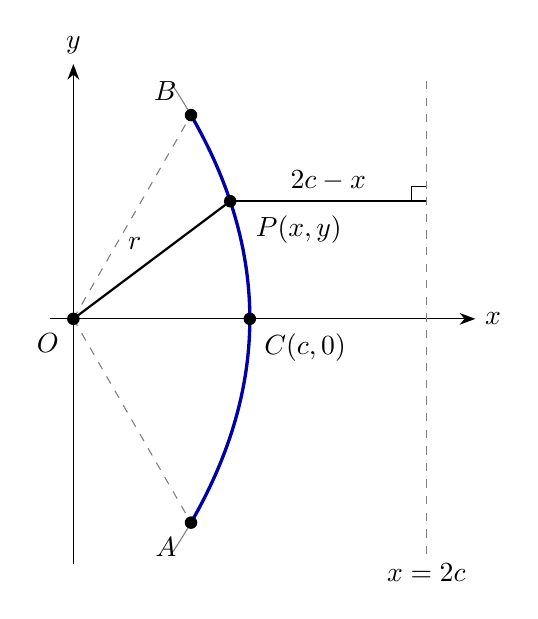
\begin{tikzpicture}[scale=.83]
\def\cc{2.7}\def\endY{3.117691454}
\coordinate (O) at (0,0);\coordinate (C) at (\cc,0);
\coordinate (A) at (1.8,-\endY);\coordinate (B) at (1.8,\endY);
\coordinate (P) at (2.4,1.8);\coordinate (D) at (5.4,1.8);
\draw[axis] (-.35,0)--(6.15,0) node[right] {$x$};
\draw[axis] (0,-3.75)--(0,3.9) node[above] {$y$};
\draw[gray,dashed] (5.4,-3.6)--(5.4,3.65);
\node[below] at (5.4,-3.6) {$x=2c$};
\draw[gray] plot[domain=-3.6:3.6,samples=80,variable=\t] ({\cc-\t*\t/(4*\cc)},\t);
\draw[track] plot[domain=-\endY:\endY,samples=80,variable=\t] ({\cc-\t*\t/(4*\cc)},\t);
\draw[gray,dashed] (O)--(A);\draw[gray,dashed] (O)--(B);
\draw[thick] (O)--(P) node[midway,above left] {$r$};
\draw[thick] (P)--(D) node[midway,above] {$2c-x$};
\draw (5.18,1.8)--(5.18,2.02)--(5.4,2.02);
\node[point,label=below left:$O$] at (O) {};
\node[point,label=below right:{$C(c,0)$}] at (C) {};
\node[point,label=below left:$A$] at (A) {};
\node[point,label=above left:$B$] at (B) {};
\node[point,label={[xshift=4pt]below right:{$P(x,y)$}}] at (P) {};
\end{tikzpicture}

% map-03: X=2.3, endpoint Y=+-1.2; the half-angle plane has sqrt(length) units.
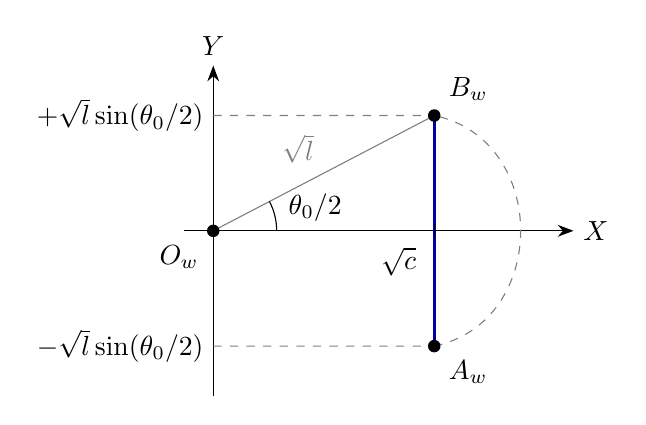
\begin{tikzpicture}[scale=1.22]
\coordinate (O) at (0,0);\coordinate (A) at (2.3,-1.2);\coordinate (B) at (2.3,1.2);
\draw[axis] (-.3,0)--(3.75,0) node[right] {$X$};
\draw[axis] (0,-1.72)--(0,1.72) node[above] {$Y$};
\draw[gray,dashed] (0,-1.2)--(A);\draw[gray,dashed] (0,1.2)--(B);
\draw[gray,dashed] (A)..controls (3.5,-.95) and (3.5,.95)..(B);
\draw[track] (A)--(B);
\draw[gray] (O)--(B) node[midway,above left] {$\sqrt l$};
\draw (.66,0) arc[start angle=0,end angle=27.5528,radius=.66];
\node at (1.06,.24) {$\theta_0/2$};
\draw (2.3,.07)--(2.3,-.07) node[below left,xshift=-3pt] {$\sqrt c$};
\node[left] at (0,1.2) {$+\sqrt l\sin(\theta_0/2)$};
\node[left] at (0,-1.2) {$-\sqrt l\sin(\theta_0/2)$};
\node[point,label=below left:$O_w$] at (O) {};
\node[point,label=below right:$A_w$] at (A) {};
\node[point,label=above right:$B_w$] at (B) {};
\end{tikzpicture}

% forces-03: c=2.5, q=0.45; arrows F/m=(x/r,y/r), N/m=(-1,0)-F/m.
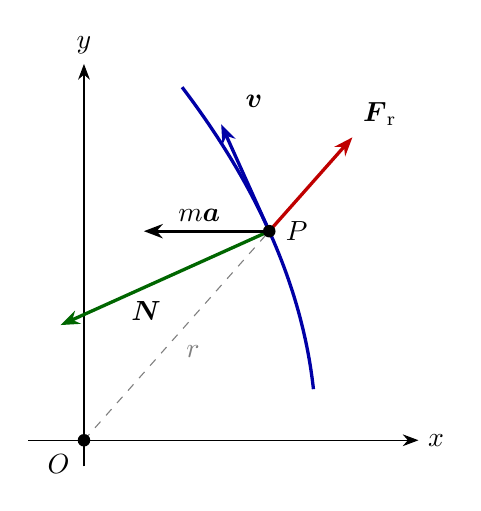
\begin{tikzpicture}[scale=1.18]
\def\cc{2.5}\def\qq{.45}\def\fs{1.35}
\coordinate (O) at (0,0);
\coordinate (P) at ({\cc*(1-\qq*\qq)},{2*\cc*\qq});
\draw[axis] (-.6,0)--(3.6,0) node[right] {$x$};
\draw[axis] (0,-.28)--(0,4.05) node[above] {$y$};
\draw[track] plot[domain=.55:3.8,samples=80,variable=\t] ({\cc-\t*\t/(4*\cc)},\t);
\draw[gray,dashed] (O)--(P) node[midway,below right] {$r$};
\draw[force,red!75!black] (P)--++({\fs*(1-\qq*\qq)/(1+\qq*\qq)},{\fs*2*\qq/(1+\qq*\qq)});
\node[above right] at (2.9,3.28) {$\boldsymbol F_{\mathrm r}$};
\draw[force,green!40!black] (P)--++({-2*\fs/(1+\qq*\qq)},{-2*\fs*\qq/(1+\qq*\qq)});
\node[below] at (.67,1.6) {$\boldsymbol N$};
\draw[force,blue!65!black] (P)--++({-1.15*\qq},1.15);
\node at (1.83,3.65) {$\boldsymbol v$};
\draw[force,black] (P)--++(-\fs,0);
\node[above] at (1.24,2.25) {$m\boldsymbol a$};
\node[point,label=below left:$O$] at (O) {};
\node[point,label=right:$P$] at (P) {};
\end{tikzpicture}
\end{document}
